\section{State of Art}
\subsection{Definitions}
In this subsection, definitions about the graph theory will be presented. Most
of the following definitions are taken from or inspired by wikipedia and
wikibook.

\subsubsection{Type of graphs}
\paragraph{Undirected simple graphs :}
An undirected simple graph is a mathematical objects composed of a set of
vertices $V$ and a set of edges $E$ and is noted $G = (V,E)$.

%TODO eventually ref for other names in Diestel
\paragraph{}
A vertex is a mathematical objects which might virtually represent anything.

\paragraph{}
An edge is an unordered pair of different vertices and is noted $\{u,v\}$,
sometimes it can also be contracted to the following notation $uv$.

\begin{figure}[!h]
  \begin{center}
    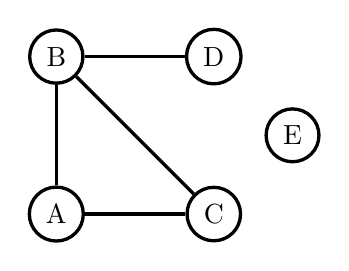
\begin{tikzpicture}[scale=0.5]
  \node[draw,circle, very thick] (A) at (2,0) {A};
  \node[draw,circle, very thick] (B) at (2,4) {B};
  \node[draw,circle, very thick] (C) at (6,0) {C};
  \node[draw,circle, very thick] (D) at (6,4) {D};
  \node[draw,circle, very thick] (E) at (8,2) {E};
  \draw[very thick] (A) -- (B);
  \draw[very thick] (B) -- (D);
  \draw[very thick] (C) -- (B);
  \draw[very thick] (C) -- (A);
\end{tikzpicture}

  \end{center}
  \caption{An undirected simple graph with 5 vertices and 4 edges}
\end{figure}

%TODO source + dst
\paragraph{Directed graphs :} 
A directed simple graph is a graph with edges defined as ordered pairs
$e = (u,v)$ rather than a two-element set $e = \{u,v\}$.
\begin{figure}[!h]
  \begin{center}
    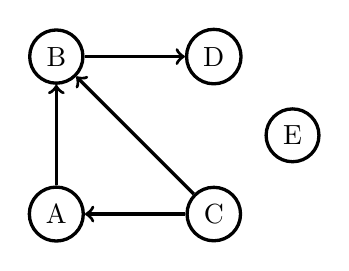
\begin{tikzpicture}[scale=0.5]
 \tikzset{directed/.style={->}} 
  \node[draw,circle, very thick] (A) at (2,0) {A};
  \node[draw,circle, very thick] (B) at (2,4) {B};
  \node[draw,circle, very thick] (C) at (6,0) {C};
  \node[draw,circle, very thick] (D) at (6,4) {D};
  \node[draw,circle, very thick] (E) at (8,2) {E};
  \draw[very thick, directed] (A) -- (B);
  \draw[very thick, directed] (B) -- (D);
  \draw[very thick, directed] (C) -- (B);
  \draw[very thick, directed] (C) -- (A);
\end{tikzpicture}

  \end{center}
  \caption{A directed simple graph with 5 vertices and 4 edges}
\end{figure}

\paragraph{Subgraphs :}
Given a graph $G = (V,E)$ and a graph $G' = (V',E')$, $G'$ is a subgraph of $G$ 
if and only if $V \subseteq V'$ and $E \subseteq E'$.

\begin{figure}[!h]
  \begin{center}
    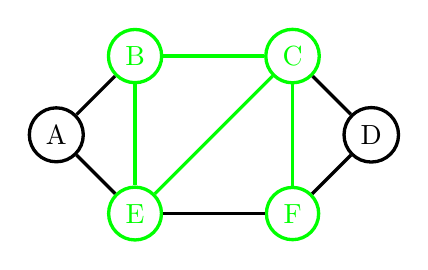
\begin{tikzpicture}[scale=0.5]
  \node[draw,circle, very thick] (A) at (0,2) {A};
  \node[draw,circle, very thick, color=green] (B) at (2,4) {B};
  \node[draw,circle, very thick, color=green] (C) at (6,4) {C};
  \node[draw,circle, very thick] (D) at (8,2) {D};
  \node[draw,circle, very thick, color=green] (E) at (2,0) {E};
  \node[draw,circle, very thick, color=green] (F) at (6,0) {F};
  \draw[very thick] (A) -- (B);
  \draw[very thick] (A) -- (E);
  \draw[very thick, color=green] (B) -- (C);
  \draw[very thick, color=green] (B) -- (E);
  \draw[very thick] (C) -- (D);
  \draw[very thick, color=green] (C) -- (E);
  \draw[very thick, color=green] (C) -- (F);
  \draw[very thick] (D) -- (F);
  \draw[very thick] (E) -- (F);
\end{tikzpicture}

  \end{center}
  \caption{A graph and one of his subgraph (in green)}
\end{figure}

\paragraph{Tree :}
A tree is an undirected simple connected\footnote{See \ref{defConnectivity}}
graph.

\begin{figure}[!h]
  \begin{center}
    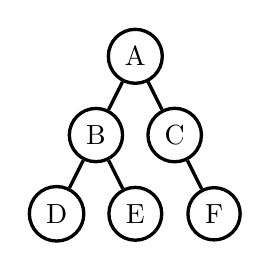
\begin{tikzpicture}[scale=0.5]
  \node[draw,circle, very thick] (A) at (2,4) {A};
  \node[draw,circle, very thick] (B) at (1,2) {B};
  \node[draw,circle, very thick] (C) at (3,2) {C};
  \node[draw,circle, very thick] (D) at (0,0) {D};
  \node[draw,circle, very thick] (E) at (2,0) {E};
  \node[draw,circle, very thick] (F) at (4,0) {F};
  \draw[very thick] (A) -- (B);
  \draw[very thick] (A) -- (C);
  \draw[very thick] (B) -- (D);
  \draw[very thick] (B) -- (E);
  \draw[very thick] (C) -- (F);
\end{tikzpicture}

  \end{center}
  \caption{A tree}
\end{figure}

\paragraph{Spanning Tree :}
A tree $T$ is a spanning tree of a graph $G$ if it includes every vertex of $G$ 
and is a subgraph of $G$.

\begin{figure}[!h]
  \begin{center}
    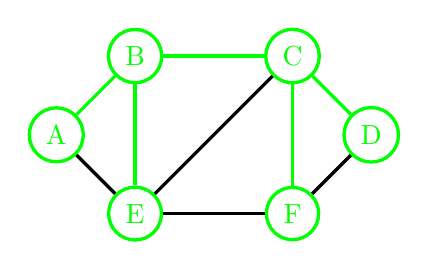
\begin{tikzpicture}[scale=0.5]
  \node[draw,circle, very thick, color=green] (A) at (0,2) {A};
  \node[draw,circle, very thick, color=green] (B) at (2,4) {B};
  \node[draw,circle, very thick, color=green] (C) at (6,4) {C};
  \node[draw,circle, very thick, color=green] (D) at (8,2) {D};
  \node[draw,circle, very thick, color=green] (E) at (2,0) {E};
  \node[draw,circle, very thick, color=green] (F) at (6,0) {F};
  \draw[very thick, color=green] (A) -- (B);
  \draw[very thick] (A) -- (E);
  \draw[very thick, color=green] (B) -- (C);
  \draw[very thick, color=green] (B) -- (E);
  \draw[very thick, color=green] (C) -- (D);
  \draw[very thick] (C) -- (E);
  \draw[very thick, color=green] (C) -- (F);
  \draw[very thick] (D) -- (F);
  \draw[very thick] (E) -- (F);
\end{tikzpicture}

  \end{center}
  \caption{A spanning tree (in green)}
\end{figure}

\subsubsection{Fundamentals notation}
\paragraph{Graph Size :}
The size of a graph $G$ is its number of edges, i.e. $|E(G)|$.

\paragraph{Graph order :}
The order of a graph $G$ is its number of vertices, i.e. $|V(G)|$.

\paragraph{Adjacent :}
Two vertices, $u$ and $v$, are adjacent in a simple graph $G$, if and only if
there's an edge of $G$ which contains $u$ and $v$, i.e. $\{u,v\} \in E(G)$.

\paragraph{Vertex degree :}
The degree of a vertex in a simple undirected graph is equal to the number of
vertices adjacent to it.

\subsubsection{Path}
\paragraph{Path :}
From~\cite{Diestel} :\\
A path is a non-empty graph $P = (V, E)$ of the form
$$ V = \{x_0,x_1, \dots, x_k \} \;\;\; E=\{x_0x_1, x_1x_2, \dots, x_{k-1}x_k \}$$
where the $x_i$ are all distinct. The vertices $x_0$ and $x_k$ are {\em linked}
by $P$ and are called its {\em ends}; the vertices $x_1, \dots, x_{k-1}$ are the
{\em inner} vertices of $P$. The number of {\em edges} of path is its
{\em length}, and the path of length $k$ is denoted by $P^k$. Note that $k$ is
allowed to be zero; thus, $P^0 = K^1$.
%TODO : explains K before

\begin{figure}[!h]
  \begin{center}
    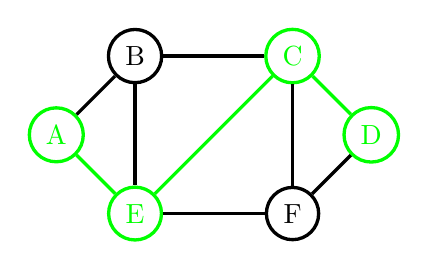
\begin{tikzpicture}[scale=0.5]
  \node[draw,circle, very thick, color=green] (A) at (0,2) {A};
  \node[draw,circle, very thick] (B) at (2,4) {B};
  \node[draw,circle, very thick, color=green] (C) at (6,4) {C};
  \node[draw,circle, very thick, color=green] (D) at (8,2) {D};
  \node[draw,circle, very thick, color=green] (E) at (2,0) {E};
  \node[draw,circle, very thick] (F) at (6,0) {F};
  \draw[very thick] (A) -- (B);
  \draw[very thick, color=green] (A) -- (E);
  \draw[very thick] (B) -- (C);
  \draw[very thick] (B) -- (E);
  \draw[very thick, color=green] (C) -- (D);
  \draw[very thick, color=green] (C) -- (E);
  \draw[very thick] (C) -- (F);
  \draw[very thick] (D) -- (F);
  \draw[very thick] (E) -- (F);
\end{tikzpicture}

  \end{center}
  \caption{A path of length 4 (in green)}
\end{figure}

\subsubsection{Cuts}
Let $G=(V,E)$ be a graph.
\paragraph{Cut :}
A cut $C=(S,T)$ is a partition of $V$ into two disjoint subsets that are joined by at least one edge.

\paragraph{Cut-set :}
The cut-set of a cut $C=(S,T)$ is the set of edge defined as $\{(u,v)\in E | u\in S, v \in T\}$.

\paragraph{Cut Size :}
The size of a cut is the number of edges in the cut-set.

\begin{figure}[!h]
  \begin{center}
    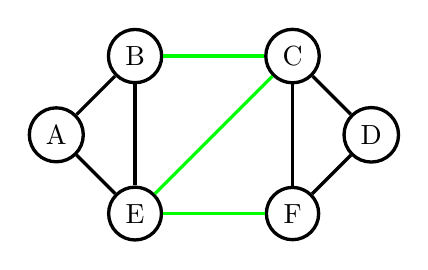
\begin{tikzpicture}[scale=0.5]
  \node[draw,circle, very thick] (A) at (0,2) {A};
  \node[draw,circle, very thick] (B) at (2,4) {B};
  \node[draw,circle, very thick] (C) at (6,4) {C};
  \node[draw,circle, very thick] (D) at (8,2) {D};
  \node[draw,circle, very thick] (E) at (2,0) {E};
  \node[draw,circle, very thick] (F) at (6,0) {F};
  \draw[very thick] (A) -- (B);
  \draw[very thick] (A) -- (E);
  \draw[very thick, color=green] (B) -- (C);
  \draw[very thick] (B) -- (E);
  \draw[very thick] (C) -- (D);
  \draw[very thick, color=green] (C) -- (E);
  \draw[very thick] (C) -- (F);
  \draw[very thick] (D) -- (F);
  \draw[very thick, color=green] (E) -- (F);
\end{tikzpicture}

  \end{center}
  \caption{A cut-set (in green)}
\end{figure}

\paragraph{Minimum Cut :} 
The minimum cut is the cut with the lowest size. 

\paragraph{Vertex Cut :}
A vertex cut $C=V'$ is a subset $V'$ of $V$ such that $G-V'$ becomes
disconnected.

\begin{figure}[!h]
  \begin{center}
    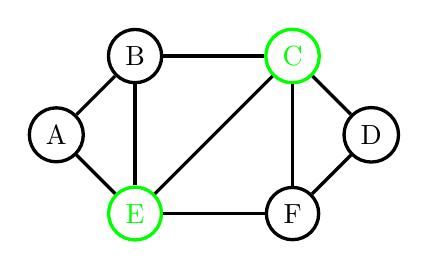
\begin{tikzpicture}[scale=0.5]
  \node[draw,circle, very thick] (A) at (0,2) {A};
  \node[draw,circle, very thick] (B) at (2,4) {B};
  \node[draw,circle, very thick, color=green] (C) at (6,4) {C};
  \node[draw,circle, very thick] (D) at (8,2) {D};
  \node[draw,circle, very thick, color=green] (E) at (2,0) {E};
  \node[draw,circle, very thick] (F) at (6,0) {F};
  \draw[very thick] (A) -- (B);
  \draw[very thick] (A) -- (E);
  \draw[very thick] (B) -- (C);
  \draw[very thick] (B) -- (E);
  \draw[very thick] (C) -- (D);
  \draw[very thick] (C) -- (E);
  \draw[very thick] (C) -- (F);
  \draw[very thick] (D) -- (F);
  \draw[very thick] (E) -- (F);
\end{tikzpicture}

  \end{center}
  \caption{A vertex cut (in green)}
\end{figure}


\paragraph{Vertex Cut Size :}
The size of the  vertex cut is the size of the subset $V'$

\paragraph{Minimum Vertex Cut :}
The minimum vertex cut is the vertex cut with the lowest size.

\subsubsection{Flow}
\paragraph{Flow Network}
A flow network is a directed graph $G=(V,E)$ whose edges have a non-negative
capacity, i.e. $\forall (u,v) \in E(G), c(u,v) \geq 0$.

\begin{figure}[!h]
  \begin{center}
    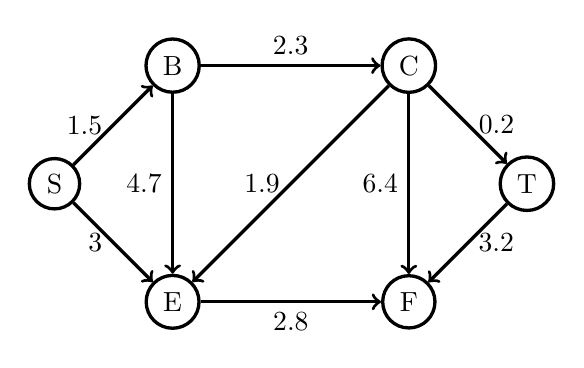
\begin{tikzpicture}[scale=0.5]
 \tikzset{directed/.style={->}} 
  \node[draw,circle, very thick] (A) at (0,3) {S};
  \node[draw,circle, very thick] (B) at (3,6) {B};
  \node[draw,circle, very thick] (C) at (9,6) {C};
  \node[draw,circle, very thick] (D) at (12,3) {T};
  \node[draw,circle, very thick] (E) at (3,0) {E};
  \node[draw,circle, very thick] (F) at (9,0) {F};
  \draw[very thick, directed] (A) -- node[left] {1.5} (B) ;
  \draw[very thick, directed] (A) -- node[left] {3} (E);
  \draw[very thick, directed] (B) -- node[above] {2.3} (C);
  \draw[very thick, directed] (B) -- node[left] {4.7} (E);
  \draw[very thick, directed] (C) -- node[right] {0.2} (D);
  \draw[very thick, directed] (C) -- node[left] {1.9} (E);
  \draw[very thick, directed] (C) -- node[left] {6.4} (F);
  \draw[very thick, directed] (D) -- node[right] {3.2} (F);
  \draw[very thick, directed] (E) -- node[below] {2.8} (F);
\end{tikzpicture}

  \end{center}
  \caption{A flow network}
\end{figure}

\paragraph{Flow :}
Let we distinguish two vertices: a source $s$ and a sink $t$.
A flow is a fonction which associate to each edge $(u,v) \in E$ a real:
$f: V \times V \rightarrow \mathbb{R}$ such as:
\begin{itemize}
    \item Capacity constraints : $\forall (u,v) \in E, f(u,v) \leq c(u,v)$
    \item Symetry : $\forall (u,v) \in E, f(u,v) = - f(v,u) $
    \item Flow conservation: $\forall u \in V - \{s,t\}, \sum_{v \in V}f(u,v) = 0$ 
\end{itemize}


\paragraph{Maximum-flow Minimum-cut Theorem :}
The max-flow min-cut theorem states that in a flow network, the maximum amount
of flow passing from the source node to the sink node is equal to the capacity
of the minimum cut.


\subsubsection{Connectivity}
\paragraph{Connectivity :}\label{defConnectivity}
A graph is {\em connected} if for every pair $(u,v)$ of vertices from the
graph, a path exists from $u$ to $v$. Otherwise, the graph is {\em unconnected}.

\paragraph{k-connexity :}
A graph with at least $k+1$ vertices is $k$ connex, if for every pair of
vertices, there is at least $k$ vertex disjoint paths between these vertices.
%TODO define vertex disjoint paths before
Another definition could be: a graph is $k$-connex if it's minimal vertex cut
is of a size less or equal to $k$.

\paragraph{k-connectivity :}
A graph is $k$-connected if it is $k$-connex and not $k+1$-connex. 

\begin{figure}[!h]
  \begin{center}
    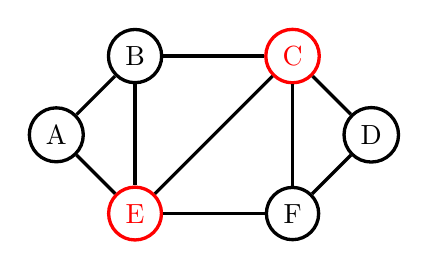
\begin{tikzpicture}[scale=0.5]
  \node[draw,circle, very thick] (A) at (0,2) {A};
  \node[draw,circle, very thick] (B) at (2,4) {B};
  \node[draw,circle, very thick, color=red] (C) at (6,4) {C};
  \node[draw,circle, very thick] (D) at (8,2) {D};
  \node[draw,circle, very thick, color=red] (E) at (2,0) {E};
  \node[draw,circle, very thick] (F) at (6,0) {F};
  \draw[very thick] (A) -- (B);
  \draw[very thick] (A) -- (E);
  \draw[very thick] (B) -- (C);
  \draw[very thick] (B) -- (E);
  \draw[very thick] (C) -- (D);
  \draw[very thick] (C) -- (E);
  \draw[very thick] (C) -- (F);
  \draw[very thick] (D) -- (F);
  \draw[very thick] (E) -- (F);
\end{tikzpicture}

  \end{center}
  \caption{A 2-connected graph}
\end{figure}

\paragraph{Menger's theorem :}
The menger's theorem is an important theorem concerning connectivity.
It states the following fact:

Let G be a undirected graph and a and b two distinct vertices.
Then the size of the minimun edge cut for a and b is equal to the maximun number of pairwise node-independent paths from a to b.


\subsubsection{Partition}
\paragraph{k-partition :}
A set $\{V_1,...,V_k\}$ is a k-partition:
\begin{itemize}
    \item $\forall i, \lceil V_i \rceil$ is connected
    \item $\sum\limits_{i=0}^k|V_i| = |V|$
    \item $\forall i,j \in \{1, \dots, k\}^2, i \neq j, V_i \cap V_j = \emptyset$
\end{itemize}

\begin{figure}[!h]
    \begin{center}
        
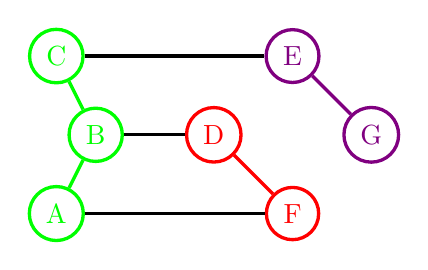
\begin{tikzpicture}[scale=0.5]
  \node[draw,circle, very thick, color=green] (A) at (0,0) {A};
  \node[draw,circle, very thick, color=green] (B) at (1,2) {B};
  \node[draw,circle, very thick, color=green] (C) at (0,4) {C};
  \node[draw,circle, very thick, color=red] (D) at (4,2) {D};
  \node[draw,circle, very thick, color=violet] (E) at (6,4) {E};
  \node[draw,circle, very thick, color=red] (F) at (6,0) {F};
  \node[draw,circle, very thick, color=violet] (G) at (8,2) {G};
  \draw[color=green, very thick] (A) -- (B);
  \draw[color=green, very thick] (B) -- (C);
  \draw[very thick] (B) -- (D);
  \draw[very thick] (A) -- (F);
  \draw[very thick] (C) -- (E);
  \draw[very thick, color=violet] (E) -- (G);
  \draw[very thick, color=red] (D) -- (F);
\end{tikzpicture}

    \end{center}
    \caption{A 3-partition graph}
\end{figure}

\subsection{Algorithme}
\subsubsection{k-connectivity}
\paragraph{}
As we have seen in the previous section, the connectivty of a graph is equal to the size of the smallest subset wich disconnect the graph.
To do so the max-flow min-cut theorem states that the maximun flow between to vertices is equal to the minimun cut to disconect this to vertices.
But if we use directly a flow algorithm, we will compute the edge-connectivity and not the vertex-connectivity.

So first the graph need to be transform. We need capacity on the nodes. To do so each nodes will be divided into two new nodes. Each incomming edge will be attach to the first node and each leaving edge to the second node. Another edge will be add between the two new node.
The capacity of all edge of the graph will be set to 1.

Then to find the connectivity, we compute the maximun flow between each pair of nodes and we keep only the lowest value. This value is the connecivity.


\begin{algorithm}[!h]
    \KwData{$G=(V,E)$ a graph}
    \KwResult{$k$ the connecitvity}
    $min = \infty$\;
    $G^{'} = TransformNode(G)$\;
    \ForAll{$u,v \in V, u \neq v, (u,v) \notin E$}{
        $f = maximunFlow(G^{'},u,v)$\;
        \If{$f < min$}{
            $min = f$\;
    }
}
    \Return{$min$}\;
    \caption{Compute the connecitvity}
\end{algorithm}

\subsubsection{k-partitioning}
In this section, we are going to focus on the differents existing k-partitioning algorithms.
First of all, for a general graph G, finding a k-partition is a NP-hard problem\cite{Dyer1985139}.
So for now no general polynomial algorithms has been found.
So we are going to focus on paricular graph.

It has been proven that for a k-connected graph G a k-partition exists\cite{GE78,LL77}.
Arcoding to the article, there are polynomial solutions for $k=2$\cite{GE78,LL77} and $k=3$.

If G is a planar graph, there is a linear-time algorithm for $k = 4$ \cite{Nakano1997315}.




